\documentclass[12pt]{article}

\usepackage{times}
\usepackage[final]{changes}
\usepackage{amssymb}
\usepackage{graphicx}
\usepackage{amsmath,amssymb,latexsym,float,epsfig,subfigure}
\usepackage{mathtools, bbm}
\usepackage{amsmath} % assumes amsmath package installed
\usepackage{amssymb}  % assumes amsmath package installed
\usepackage{lipsum}
\usepackage[export]{adjustbox}
\usepackage[normalem]{ulem} % underline
\usepackage{wrapfig}
\usepackage{multirow}
\usepackage{balance}
\usepackage{color}
\usepackage{url}
\usepackage{microtype}
\usepackage{array}
\usepackage{algorithm, algorithmic}
\usepackage{breqn}
\usepackage{setspace}
\usepackage[bottom]{footmisc}

%\doublespacing

\newcommand{\argmax}{\arg\!\max}
\newcommand{\norm}[1]{\left\lVert#1\right\rVert}
\newcommand{\DGc}[1]{{\textbf{\color{blue}{#1}}}}
\newcommand{\POINTS}[1]{{\textbf{\color{red}{#1}}}}
\definechangesauthor{de}


% <http://psl.cs.columbia.edu/phdczar/proposal.html>:
%
% The standard departmental thesis proposal format is the following:
%        30 pages
%        12 point type
%        1 inch margins all around = 6.5   inch column
%        (Total:  30 * 6.5   = 195 page-inches)
%
% For letter-size paper: 8.5 in x 11 in
% Latex Origin is 1''/1'', so measurements are relative to this.

\topmargin      0.0in
\headheight     0.0in
\headsep        0.0in
\oddsidemargin  0.0in
\evensidemargin 0.0in
\textheight     9.0in
\textwidth      6.5in

\title{{\bf Towards an Information Theoretic Framework For Human-Autonomy Interaction in Shared Control} \\
\it Thesis proposal}
\author{ {\bf Deepak Edakkattil Gopinath}  \\
Department of Mechanical Engineering \\
Northwestern University\\
{\small deepakgopinath@u.northwestern.edu}
}
\date{\today}

\begin{document}
\pagestyle{plain}
\pagenumbering{roman}
\maketitle

\pagebreak
\begin{abstract}
Human-Autonomy Interaction (HAI) in the context of shared-control robotics is a rich and complex phenomenon. The effectiveness and usefulness of shared-control human-machine systems critically depends on the fluency and efficacy of human-robot interaction. Efficient HAI can lead to an improvement in joint task performance with higher user satisfaction and enhanced trust, all of which are desired characteristics of a joint human-machine system. From an engineer/system designer's perspective, in order to achieve optimal performance the design of autonomy should adequately taken into account the richness, subtleties and complexity of the interaction between the human and the machine.

In this thesis proposal, I plan to propose a mathematical framework for human-autonomy interaction for shared-control robotics utilizing ideas from \textit{probabilistic graphical models} and \textit{information theory}. More specifically, the interaction between human and autonomy will be modeled as coupled perception-action loops unfolding in time using \textit{causal Bayesian Networks}. Within this framework of causal Bayesian Networks, design of autonomy can be thought of as appropriately timed \textit{interventions} at specific parts of model, with an intention to alter the bi-directional information flow between the human and machine. Using the proposed mathematical model, I will research three important problems that arise in HAI namely, a) \textbf{quantification of transparency}, b) \textbf{improvement of human skill acquisition} and c) \textbf{enhancement	 of overall task performance and autonomy's inference capabilities}. The eventual goal is to utilize the proposed mathematical framework to inform the design of autonomy that will help \textit{quantify transparency levels in a given interaction scenario}, \textit{facilitate human learning}, and \textit{enhance task performance and inference accuracy}.
\end{abstract}

\pagebreak
\tableofcontents
\pagebreak

\cleardoublepage
\pagenumbering{arabic}

\section{Introduction}
\label{sec:intro}
%How robots and machines are ubiquitous in our society?

Robots are ubiquitous in the modern-day society and have revolutionized the relationship between man and machine. Compared to a few decades ago, in the present day, robots have transitioned out of the rigid, structured and specialized industrial environments to the more rich, complex and unpredictable day-to-day human environments and have impacted diverse domains of human endeavor such as healthcare~\cite{laplante1992assistive}, entertainment~\cite{gopinath2016generative} and home robotics~\cite{fischinger2016hobbit}.


The impact is even more significant in the domain of assistive and rehabilitation robotics in which the potential to drastically enhance the quality of life for people suffering from motor impairments as a result of spinal cord or brain injuries is immense~\cite{muelling2017autonomy}. Devices such as smart wheelchairs, exoskeletons and assistive robotic arms can help to promote independence, boost self-esteem and help to extend mobility and manipulation capabilities of motor-impaired individuals and can revolutionize how they interact with society~\cite{mataric2007socially}.

%
%\noindent What is their potential? Specific application in the domain of assistive robotics.
%One on end of the spectrum robots are passive machines that can perform some task by manual teleoperation by the user. On the other end, we have full autonomy in which the human does not play an active role in task execution. 
%
%\noindent What is shared autonomy?
The standard usage of these assistive machines, however, still relies on manual teleoperation by the human typically enacted through a control interface such as a joystick or a switch-based headarray; that is, in such scenarios robots are not endowed with any intelligence and are treated as \textit{passive} machines that function as extensions of human motor abilities~\cite{simpson2008tooth}. However, one of the most difficult conundrums is that greater the motor impairment of the user, the more limited the interfaces that are available for them to use. As a result, control of these machines can become extremely difficult due to the low dimensionality, sparsity and bandwidth of the control interfaces and are further exacerbated by the inherent complexity in robot dynamics and the physical limitations of the users~\cite{pilarski2012dynamic}.
In such cases, \textit{robot autonomy}, the ability of robots to accomplish a task independently without requiring explicit instructions from a human, holds considerable promise as a tool to offset (and in some cases restore) the above-mentioned limitations. Advances in the fields of machine learning and artificial intelligence have helped to endow these assistive machines with better decision making and prediction capabilities while interacting with humans in real-world scenarios~\cite{huang2015using}.
However, in literature there is a growing consensus that users of assistive technologies \textit{do not} prefer to cede full control authority to the robotic partner during task execution~\cite{gopinath2017human}. In such cases, the introduction of \textit{shared control} seeks to find a middle ground between full teleoperation and autonomy by offloading only some aspects of task execution to the autonomy~\cite{wasson2003user, demeester2008user}. 

In a shared-control system, the task responsibility is split between the user and autonomy with the aim of reducing human effort in accomplishing a task. Human-Autonomy Interaction (HAI)\footnote{Human-Autonomy Interaction is closely related to Human-Robot Interaction. However, in this proposal, we interpret the term `robot' as an embodied physical entity that exists in the world and `autonomy' as the intelligence that gives the robot a sense of agency. In the context of shared-control, human and autonomy jointly control the robot to accomplish tasks in a coordinated manner. The underlying interaction is between human and autonomy, hence the term HAI.} in the context of shared-control is a rich and complex phenomena. The effectiveness and usefulness of shared-control human-machine systems critically depends on the quality and efficiency of HAI. That is, for robots and humans to work side-by-side and achieve joint goals and accomplish various tasks in a \textit{coordinated} and \textit{cooperative} manner, it is imperative that both parties understand each other, communicate and infer internal desires and intentions efficiently~\cite{hoc2001towards}. From an engineering perspective, design of appropriate kinds of autonomous behaviors for a shared-control system, therefore, needs to take into account the dynamics of HAI during the course of task execution~\cite{hoffman2007cost}. 

Current research approaches for design of shared-control systems rely on various kinds of mathematical models to solve different aspects of HAI as independent subproblems and therefore suffer from generalization across tasks, robotic platforms and user types. For my thesis, I am motivated by the desire to develop a \textit{unified} mathematical framework to analyze different aspects of HAI under a single umbrella in an attempt to shed light on the more \textit{fundamental} and \textit{low-level} characteristics of human-robot teaming.

To that end, I propose a mathematical framework that models HAI in the context of shared-control utilizing ideas from \textit{probabilistic graphical models}~\cite{koller2009probabilistic} and \textit{information theory}~\cite{cover2012elements}. More specifically, the interaction will be modeled as \textit{coupled perception-action loops} unfolding in time using \textit{causal Bayesian Networks}~\cite{pearl2009causality}. The nodes in the network will represent the different variables (both latent and observed) that are relevant for the model and the edges represent the probabilistic influence they have on each other. In an attempt to quantify the fluency, transparency and cooperation levels that characterize the interaction, emphasis will be placed on analyzing the \textit{information flow} between the nodes in the network~\cite{ay2008information}. Within this proposed framework of causal Bayesian networks, design of autonomy can be thought of as appropriately timed \textit{interventions} that have the potential to alter bidirectional information flow between human and autonomy.
Our hypothesis is that \textit{information flow} is a more fundamental and low-level descriptor of interaction dynamics and joint system performance that system designers should focus on when designing autonomous behaviors.
% Efficient task performance, enhanced coordination and transparency can benefit from improved bidirectional information flow between autonomy and humans\DGc{R}.  
Using the proposed model, I intend to address three main subproblems relevant to shared autonomy namely, \textit{learning}, \textit{inference} and \textit{task performance}.

The first research question (\textbf{RQ1}) that I will address in my work concerns the quantification of transparency of HAI in a given interaction scenario. In a human-robot team, transparency can be thought of as the \textit{observability} and \textit{predictability} of either agent's behavior; it can also refer to the effective and legible bi-directional communication of internal desires, goals and intentions which in turn facilitates and promotes cooperation and coordinated task execution. The effectiveness and usefulness of shared-control system critically depend on the fluency and transparency of HAI. In \textbf{RQ1}, I will utilize the notion of information flow in Bayesian Networks as measured by \textit{multivariate transfer entropy} to characterize robot-to-human and human-to-robot transparency directly from sensor measurements.  Transfer entropy is a directed information-theoretic metric that aims to capture directed information flow/transfer from a source random process to a target random process~\cite{schreiber2000measuring}. Higher transfer entropy implies that knowledge of the source process's past state improves the predictability of the target process's future state. In a joint task setting, if the robot behavior is more transparent to the human, the information regarding the autonomy's intention will be utilized properly by the human, who will likely act in a more predictable manner. In such cases, transfer entropy can become a viable metric to capture the increase in predictability, caused by higher transparency. 

The second research question (\textbf{RQ2}) that I will address in my thesis is \textit{how can autonomy help humans learn robot dynamics better}.   A greater skill level typically enables the users to express their intentions more clearly thereby improving human-to-robot transparency. When a human interacts with a machine in a shared-control setting, both parties are continually learning about each others' intentions, plans and actions~\cite{ikemoto2012physical}. For example, for novice users familiarity with the device and knowledge about the dynamics of the control interface and the robot increase with extensive training and practice~\cite{mussaivaldi2000motor}. The initial forward (and inverse) kinematics (or dynamics) model that the user maintains internally at the beginning of training might be drastically different from the true underlying system kinematics (or dynamics). Due to learning effects, the internal model will likely become closer to the true model. However, the learning strategies that humans adopt need not always be optimal, for example, users might not explore the state and action space in an efficient and exhaustive manner and therefore can erroneously extrapolate the learned internal model between different regions of the workspace. In \textbf{RQ2}, we are motivated by ideas from \textit{curriculum learning}[cite bengio] and we seek to develop an algorithm that guides the user towards regions of the state space that exhibit highly nonlinear kinematics or require more cognitive resources to teleoperate. To this end, we will rely on data-driven methods to generate  \textit{information density maps} that quantify the temporal and spatial aspects of how humans explore the state space during self-guided training and task execution. The autonomy will then sample `training zones' according the information density map and nudge the users such that their exploration trajectories during autonomy-guided training become maximally ergodic with respect to the information density map thereby gaining more `practice time' in those parts of the state space where robot control is hard. Therefore, autonomy can play the role of a \textit{informative teacher} and help the human in skill acquisition and provide appropriate guidance during the learning process. Potentially, this can have a significant impact in the design of training procedures for new users of assistive robots, thereby improving the baseline above which the assistance provided by autonomy can become more effective. 
%This is important because the effectiveness of autonomy assistance is higher when the user has already developed a considerable amount of skill in robot control.

Once transparency is quantified (\textbf{RQ1}) and users have gained sufficient skill (as a result of \textbf{RQ2}), in my last research question (\textbf{RQ3}), I will shift my focus to the design on autonomy that optimizes transparency of HAI in a shared-control setting. Typical design of autonomy for shared-control systems aims to improve various objective aspects of joint task performance, such as task completion times, energy consumption and inference accuracy. Optimization-based techniques are used to derive autonomy's policy, in which the cost functions that capture desired behavior are pre-specified by the system designer~\cite{javdani2015shared}. However, in the domain of assistive shared-control, subjective metrics, such as user satisfaction, comfort and trust, are also of paramount importance for successful adoption of these technologies~\cite{kim2012autonomy}. Determining the exact mathematical structure for the cost function that incorporates these subjective metrics is likely an intractable problem~\cite{gopinath2017human}. In \textbf{RQ3}, rather than focusing on the objective or subjective metrics independently, we intend to focus on the optimization of bi-directional information flow between human and autonomy. The hypothesis is that this optimization procedure will likely result in better communication of latent internal states, thereby guiding the evolution of the joint human-autonomy system towards states with higher transparency. This will result in a common ground~\cite{kiesler2005fostering} for joint task execution, which will lead to enhanced cooperation, coordination and mutual trust. The hypothesis is that, as a result of these enhancements, the desired objective and subjective outcomes (improved task performance, enhanced inference accuracy, higher user satisfaction \textit{et cetera}) will likely emerge.
%We will use measure of ergodicity to characterize the temporal and spatial aspects of state-space exploration during the learning process resulting in an information density map that will reveal the cognitively hard regions in the state space. Inspired by ideas from curriculum learning, autonomy can then sample `training zones' using the information density map such that subsequent exploration of the state space in and around the training zone will help the user with maximal skill acquisition. 

%Inherent limitations of the control interface and motor impairments can possibly put an upper bound to skill level that can be acquired. In such scenarios, the need for autonomy for task execution becomes inevitable. However, any successful assistive robotic system needs to have a good idea of the user's needs and intentions. That is, \textit{user intent inference} is a necessary and crucial component to ensure proper assistance~\cite{wang2013probabilistic}. Therefore, the second research question (\textbf{RQ2}) that I will address in my thesis is \textit{how can autonomy assistance be designed so that inference becomes more accurate}. Typically, the user's internal state (desires, goals and intentions) is latent (if not fully, partially) from autonomy's perspective~\cite{kelley2008understanding}. In a shared control setting inference is not a unidirectional phenomena. For example, from the users' perspective the internal logic with which autonomy helps them is not always explicitly known and therefore needs to be inferred as well. User satisfaction and acceptance heavily depends on the user's understanding of how the autonomy works. In this thesis, I plan to utilize the proposed mathematical model to reason about and shape the information flow from the user's internal state to autonomy to improve the inference accuracy. 

%In addition to facilitating learning (\textbf{RQ1}), and improving inference accuracy (\textbf{RQ2}), autonomy has to work in conjunction with the human to perform the task optimally. Therefore, the third and final research question (\textbf{RQ3}) that I hope to tackle in this thesis is \textit{how to design autonomy assistance to ensure optimal task performance}. Typically, both subjective (user satisfaction, acceptance, trust) and objective metrics (task completion time, number of mode switches) equally inform the optimality criteria~\cite{gopinath2017human}. Rather than focusing on the above-mentioned metrics independently, in this thesis work I will focus on optimal bidirectional information flow between the human and autonomy. The hypothesis is that optimization of information flow between the autonomy and human will likely result in better communication of latent internal states thereby leading to a common ground for joint task execution. This will likely lead to enhanced cooperation and mutual understanding as a result of which the desired outcomes (better task performance, improved user satisfaction) will likely naturally emerge.

In summary, in this proposed thesis I intend to develop a mathematical framework to model HAI within shared autonomy and plan to research solutions to the questions presented above (\textbf{RQ1}, \textbf{RQ2} and \textbf{RQ3}). I am motivated by the need to develop a unified theoretical framework for shared autonomy. This work will be the first to treat information content and flow as the key components in understanding the dynamics of interaction between human and autonomy during task execution and training. More importantly, this work proposes a fundamentally different way of thinking about autonomy; one in which \textit{autonomy is a exogenous intervention that alters the information flow in a coupled perception-action loop to bring about desired outcomes during task execution or learning}.
%\POINTS{A paragraph on LEARNING}

%\POINTS{A paragraph on INFERENCE mechanisms}

%\POINTS{A paragraph on TASK PERFORMANCE}

%\POINTS{Closing Paragraph}
%
%\POINTS{For robots to work alongside humans to help humans and achieve joint goals, requires that both parties understand each other and work together balha blah. Calls for proper analysis of the phenomena}

%\POINTS{HRI is complex. Different types of phenomena unfolds. Maybe picture from presentation talking about the different types of situations. Learning, Inference, Trust, Task Performance. }

%\POINTS{Robotics holds tremendous potential for benefiting every domain of human life. Although this benefit has been limited to very specialized environments such as factories, technology has matured to integrate robotic technologies into the human environment for everyday use. However, this integration cannot be successful without understanding the interaction between robots and humans. Dr. Bilge Mutlu, of the University of Wisconsin-Madison, seeks to enable the creation of acceptable, intuitive, and desirable technologies and their smooth integration by solving technical problems, creating design examples, and mapping out human expectations of and interactions with robotic technologies. By combining computational, human-centered, and design perspectives, he and his team are able to develop new guidelines, methods, and tools that help designers of robotic technologies create products and applications that will revolutionize our future.}



%\POINTS{Current work focuses on different aspects independently. Suffers from generalizability. In this proposed work, I want to investigate more fundamental and low-level underpinnings of what makes HRI successful in a task-agnostic manner. The goal is to develop a mathematical framework to analyze HRI in a shared autonomy setting. Develop a common mathematical language to talk about the various types of phenomena outlined in the Figure.By taking into account all the subtle aspects of interaction, the design of autonomy will be more informed.} 



\pagebreak

\section{Human-Autonomy Interaction in Shared Control}
\label{sec:HRI_SA}

In this chapter I present a discussion of existing literature on mathematical approaches for modeling different aspects of HAI in a shared-control system.  
I also briefly discuss how research into softer aspects of HAI such as legibility, transparency, cooperation, attention and coordination in other domains such as cognitive psychology and philosophy help guide the design of effective human-robot teaming strategies. 

%Human-robot interaction within shared autonomy is a rich, complex and multifaceted phenomena. Researchers are interested in building autonomous behaviors for robots that can satisfy various objectives such as legibility\DGc{R}, transparency\DGc{R}, task performance\DGc{R} and enhanced trust\DGc{R} and rely on various types of mathematical frameworks to understand human decision making\DGc{R}, to improve predictive capabilities\DGc{R} and inference efficiency\DGc{R}, to enhance legibility\DGc{R} and clarity of communication\DGc{R} between the agents \textit{et cetera}. In this chapter, I discuss existing mathematical approaches for shared autonomy in literature. I also briefly discussed desired characteristics of human-robot interactions are prescribed by researchers from various related fields. 

\subsection{Mathematical Models for Shared-Control}
In shared-control, complementary abilities of humans and autonomy are leveraged to jointly accomplish various tasks such that the joint system is typically more capable than either the human or the machine on their own. However, there is no one singular definition of what shared-control is. In a recent survey paper on shared control Abbink et al. defines shared control as one in which `...\textit{human(s) and robot(s) are interacting congruently in a perception-action cycle to perform a dynamic task, that either the human or the robot could execute individually under ideal circumstances}'~\cite{abbink2018topology}. More importantly, they also propose that in a shared-control system the human and robot actions should be linked by combining them into a final control action, plan or a decision and that each agent should directly perceive how its intent is influenced by the actions of other agent(s). Clearly, HAI in this context is a complex phenomenon and for robots to function properly alongside humans, it becomes imperative that they have the capability to predict their partners actions and intentions effectively using mathematical models. 

Researchers develop mathematical frameworks for various purposes; for example, to model human behavior, to learn autonomous policies from human demonstrations, to recognize objects in the environment and generate waypoints for navigation and grasp poses for manipulation, to determine control allocation and decide how the human and autonomy control commands should be arbitrated to produce the final control command. In the following subsections I present a discuss each of the above-mentioned categories in greater detail.  

\subsubsection{Models for Human Behavior}
Teamwork in a shared autonomy system is enhanced when the team members understand each other's intentions, desires and goals. However, there are particular challenges that arise in human-robot interaction due to the differences in the mental and physical capabilities of humans and robots~\cite{hiatt2017human}. Robots can deal with such challenges by maintaining models of human cognition and behavior~\cite{javdani2015shared} spanning different timescales and levels. 
%These models endow the robots with the ability to predict their teammates' actions and therefore make decisions . Thoery of mind allusion?

Hiatt et al. in~\cite{hiatt2017human} utilize `Marr's levels of analysis'~\cite{marr1982vision} to categorize models for human behavior into three distinct categories namely: computational, algorithmic and implementational.
According to the authors, categorization of human models using Marr's level of analysis clarifies what aspects of human behavior is being modeled. Computational level techniques are ideal for scenarios that benefit from the knowledge of normative behavior that humans are ought to exhibit. These models typically rely on simplistic assumption of perfectly rational behavior and treat human idiosyncrasies and deviations from the norm as observational noise. Algorithmic level analysis, on the other hand, seeks to delve into the processing constraints that agents have and how they lead to systematic errors thereby providing better insight into \textit{why} agents deviate from normative behavior. However, the algorithmic models typically work well over shorter timescales and therefore are not suited for modeling human behavior that last over longer timescales. 

Within the computational category, one of the most common methodologies is to adopt simple probabilistic models that attempt to model very low-level short-time horizon behaviors (such as reaching motions performed by humans during a manipulation task). For example, Dragan et al., assumes a framework in which the human is treated as a optimal agent that noisily optimizes a goal-dependent cost function~\cite{dragan2013policy}. This model is used by the robot to infer user's intent in which the predicted goal is the one with the lowest cost given the user's control input. Optimality principles are particularly attractive because of their success in the domain of motor control~\cite{uno1989formation} and also because they provide a principled approach to how agents ought to behave. The framework, however, requires well-defined cost functions that provide succinct description of the task at hand. Cost functions can either be hard-coded under assumptions of rationality or hand-designed by domain experts (for example, minimization of distance to goal) or can be learned from human demonstrations using techniques such as inverse reinforcement learning~\cite{ziebart2008maximum} and inverse optimal control~\cite{dvijotham2010inverse}.

In our work on human-driven customization of shared autonomy levels~\cite{gopinath2017human}, we utilize ideas from optimal control theory to model human behavior in which we assume that humans are acting optimally with respect to an \textit{unknown} cost function. We make no assumptions regarding the nature of cost function but instead provides the human the capability to customize/optimize the control allocation parameters directly. The key insight in this work is that the human has an internal representation of what s/he wants (encoded as a cost function) and therefore by having the human optimize the control allocation parameters directly, the user will tune them to his liking and preference. Similarly, our work on mode switch assistance for intent disambiguation implicitly assumes that the model for human teleoperation of the robot is one in which the human is optimizing for shortest path to goal.

Data-driven approaches utilizing conventional machine learning algorithms are also successfully used to recognize human behavior in a wide variety of domains such as social robotics~\cite{mataric2007socially} and assistive robotics~\cite{goil2013using}. More recently, data-driven approaches based on Koopman operators have also been utilized to learn models of joint human-machine systems~\cite{broad2018learning}. Koopman operator based approaches scale well to high-dimensional spaces as the computational complexity does not grow with the number of data points. 

%Knowledge-based models can also be utilized to compare human behavior against knowledge-based representations of how different tasks are typically realized in the real world. The downside is that, knowledge-based approaches assume complete domain knowledge \DGc{R}. Furthermore, the models are not robust as the domain knowledge encoded in the models need to be updated manually for slight changes in the environment and as a result struggle with human actions or intentions outside of their knowledge \DGc{R}. 

In general, computational approaches are well suited for situations in which one is primarily concerned about what the human is doing without necessarily reasoning about the underlying causes for the behavior. 

In the algorithmic category, Hidden Markov Models (HMMs) and other Markov-based approaches are common choices for modeling human behavior~\cite{kelley2008understanding}. HMMs are powerful due to their ability to express latent variables and can be used for efficient online inference of hidden states given a set of observations. An extension of HMMs that can be useful for modeling human-robot collaboration is the Partially Observable Markov Decision Process (POMDP)~\cite{taha2011pomdp}. For example, POMDP based models are used for assessing the human partner's trust in the autonomous partner~\cite{chen2018planning}. 
%Solving a POMDP amounts to the computation of the optimal policy (probability distribution over actions given state) executed by the agent~\cite{pineau2003point}. 
POMDPs can also be used by autonomy in which the human intent are treated as latent states. By performing online inference on these latent states, autonomy will have the ability to incorporate human intentions (desired goals) into its own decision making process thereby implicitly taking into account user preferences. In general, inference over latent variables in a POMDP framework is performed via Bayesian methods in which a prior distribution over the latent variables is updated via Bayes Theorem upon receiving new evidence. The choice of likelihood function, typically encodes the human's actions/preferences give a state (policy)~\cite{dragan2012formalizing}. 

In my prior work, I have relied on heuristic approaches based on simple directedness and proximity based confidence functions to estimate reaching intent in a table-top manipulation tasks~\cite{gopinath2017human}. In order to incorporate information from past states, in my previous work, I have also developed a framework for intent inference based on ideas from \textit{Dynamic Field Theory}~\cite{schoner1995dynamics} in which the time-evolution of the probability distribution over intent/goals is specified as a constrained dynamical system~\cite{gopinathdynamic}. The activation function that drives the dynamical system plays a role akin to that of the likelihood function in Bayesian approaches in that it encodes the human's preferences. Additionally, in the domain of autonomous driving, I have developed a framework to learn agent models from partial observations that will help to predict their actions from noisy observations and deduce missing information about their environment. The probabilistic models for partially observed agents are learned via IRL techniques through which we recover the agent's policy and reward structure. Within the model, efficient imputation of latent states and actions is made possible by learning specific proposal distributions\cite{gu2015neural} to be used within an Reversible Jump Markov Chain Monte Carlo (RJMCMC) sampling process~\cite{green1995reversible}. 

A generalization of HMMs, known as Dynamic Bayesian Networks (DBNs) have also been used successfully to model human robot collaboration. DBNs are attractive due to their ability to handle multi-variate, mixed-observability variables and to represent the interdependencies between them at same as well as different time slices\cite{murphy2002dynamic}. DBNs have been successfully utilized to model human beliefs, desires and learning which can then be used for intent prediction and understanding cognitive phenomena such as concept learning\cite{tahboub2006intelligent}. However, structure of DBNs need to pre-specified by a domain expert and learning the parameters requires large amounts of data. 

\subsubsection{Models for Policy Generation}

Mathematical models are also widely used for generating/learning policies responsible for generating autonomy's control actions. In addition to successful task completion, autonomy would benefit from the its actions to be legible, natural, and safe. Learning from Demonstration (LfD)~\cite{argall2009survey} provides a framework to learn autonomous policies directly from user-provided demonstration data. For example, in imitation learning (IL) paradigms can be utilized to develop end-to-end systems that can directly map a high dimensional state to actions~\cite{bojarski2016end}. A more generalizable approach is to cast the problem with the framework of inverse reinforcement learning (IRL) in which the goal of the algorithm is to recover the user's reward function~\cite{ziebart2008maximum}.  Policies that optimize long-term accumulated reward (solution to the forward reinforcement learning (RL) problem) improves the robustness and generalization capabilities of the autonomous partner. Closely related to the RL approach is to utilize control theoretic framework to derive optimal policies for a given task. Standard optimal control theory techniques are model-based, that is, they presume the existence of a dynamics model and solve for the optimal policy with respect to a specified cost function~\cite{kirk1970optimal}. State-of-the-art RL techniques, on the other hand, can be model-free and can resort to sampling-based techniques to derive optimal policies~\cite{watkins1992q}. 

Planning-based approaches such as probabilistic road maps~\cite{kavraki1996analysis} and RRT~\cite{kuffner2000rrt} are also widely used for generating motion plans (for both robotic manipulators as well as mobile robots). In addition to task accomplishment, in order to enhance user experience robot motion plans typically need to possess various other desired characteristics. HAI in shared-control can become more seamless if the autonomy is able to make its intentions legible to the user. To that end researchers have attempted to mathematically define legibility and predictability of robot motion~\cite{dragan2013legibility}. Similarly, safety is of paramount importance when robots work in close proximity to humans. Therefore behaviors such as obstacle avoidance are incorporated into navigation plans~\cite{storms2014blending}. To this end, the on-board perception system typically relies on object detection and recognition models to identify objects of interest and obstacles thereby characterizing favorable and unfavorable parts of the state space of the robot~\cite{muller2006off}. In my work with assistive robotic manipulators for table-top manipulation~\cite{gopinath2017human}, I have utilized potential fields defined in the full six degrees-of-freedom Cartesian space (task space) to generate the robot control commands. Obstacle avoidance is implemented using velocity-dependent repellers and the intended goal is modeled as the attractor. Potential fields are computationally lightweight and produces more intuitive trajectories that correspond to straight line paths in Euclidean space~\cite{khatib1986real}. More recent work from utilized ideas from differential geometry to treat obstacles as local deformation in the geometry of the workspace and aims to derive motion policies directly in a curved Riemannian workspace~\cite{ratliff2018riemannian}. The effect of the obstacle is to curve the geodesics (straight line paths) around itself as determined by the local curvature induced by the obstacle~\cite{mainprice2016warping}. 
\subsubsection{Models for Control Allocation}

In a shared control task responsibility is split between the human and autonomy. Therefore, control allocation, that is, how exactly should control be arbitrated between the human and autonomous partner, needs to implemented appropriately for desired outcomes. Different approaches exist for sharing control between the human and autonomy that depend on the application domain, user preferences and robot platform. 
Broadly speaking, shared control approaches can be broadly classified into two main categories: hierarchical and blending-based approaches.

In the hierarchical paradigm, control allocation typically occurs at the task level in which higher level task goals are entrusted with the human and the autonomy takes care of the low-level control of the robot. For example, in the assistive domain smart wheelchair users can use a click-based interface~\cite{simpson2008tooth} to a select a desired destination in the world or a laser pointer~\cite{choi2008laser} to point to a desired goal and the autonomy can generate the global as well as local plans utilizing any state-of-the-art motion planners. In the domain of table-top manipulation users can use natural language to specify the desired grasp or reach target which then combined with a object recognition and motion planning modules can produce the desired robot trajectory~\cite{broad2016towards}. 

Blending-based approaches seek to arbitrate between human and autonomy actions at the control signal level (or the policy level) directly. In~\cite{dragan2013policy} Dragan et al. introduce the policy blending formalism for shared control in which the authors propose that ``arbitration should be contextual and the should depend on the robot's confidence in itself and in the user, as well as on the particulars of the user". A commonly used arbitration scheme is one in which the final control command issued to the robot is a linear combination of human and autonomy control commands. The blending parameter can be fixed or can be a parameterized function of the context and the autonomy's confidence in its prediction of the user's intent. In our work on human-in-the-loop customization of control allocation parameters we utilize a blending-based shared control in which the linear blending factor is a function of the probability of the predicted goal (agnostic to the type of intent inference algorithm used). We assume a piecewise-linear function and under the assumption that the human is optimizing an unknown cost function, we develop an iterative procedure with which the user is able to tune the arbitration function parameters to the his/her own satisfaction and preference~\cite{gopinath2017human}. By casting shared control allocation in a broader theoretical framework, Trautman has proposed a mathematical model for probabilistic shared control in complex dynamic environments~\cite{trautman2015assistive}. In this work, the interactive relationship between the human, autonomy and the environment is modeled as a undirected graphical model. The paper also introduces the notion of an \textit{interaction} function between the operator and the autonomy that captures the ``agreeability" between the human and autonomy. For specific forms of the interaction function, Trautman is able to recover linear blending as a special case of the more general framework and shows that in general, linear blending is suboptimal with respect to the joint metric of agreeability, safety and efficiency. 

In the domain of assistive robotics, there exists yet another particularly challenging problem. The standard usage of these assistive machines relies on manual teleoperation typically enacted through a control interface such as a joystick. However, the greater the motor impairment of the user, the more limited are the interfaces available for them to use. These interfaces (for example, sip-and-puffs and switch-based head arrays) are low-dimensional, discrete interfaces that can only operate in subsets of the entire control space (referred to as \textit{control modes}). The dimensionality mismatch between the interface and the robot's controllable degrees-of-freedom (DoF) necessitates the user to switch between control modes during teleoperation and has been shown to add to the cognitive and physical burden and affects task performance negatively~\cite{pilarski2012dynamic}.
In order to offset the drop in performance due to shifting focus (also known as task switching) from the task at hand due to switching between different control modes various mode switch assistance paradigms have been proposed. A simple time-optimal mode switching scheme has shown to improve task performance~\cite{herlant2016assistive}. Machine learning techniques have been utilized to learn mappings from robot state to control modes preferred by human users~\cite{jainrobot}. Robot operation in certain control modes can also help the autonomy to infer the user's intent more accurately and confidently, especially in scenarios where autonomy's inference of user intent is exclusively informed by human's control commands issued via the limited control interfaces. To that end, in our work, on mode switch assistance for intent disambiguation we developed a disambiguation metric to characterize the intent disambiguation capabilities of a control dimension/control mode. By having the user operate the robot in the disambiguating control mode, the control commands become more \textit{intent-expressive} and as a result autonomy is able to step in and provide appropriate assistance. In this work, we also introduce the notion of \textit{inverse legibility}, in which the roles are switched and the human-generated actions \textit{help the robot} to infer human intent confidently and accurately~\cite{gopinath2017mode}. 

\subsection{Characteristics of Ideal HAI}
Humans are highly adept at working together in teams and are able to effectively coordinate and cooperate with their teammates in a seamless, natural and fluid manner in a joint task setting. How exactly are humans able to interact efficiently in a team setting?  What do humans prioritize, besides successful task accomplishment, when working alongside others? What are some fundamental characteristics of any successful team? Researchers in the fields of cognitive psychology and  philosophy have been long interested in these questions. 
%Human-robot interaction researchers and roboticists equally benefit from the insights that psychologists and philosophers have had into these questions. 

It has been widely established that one of the most essential components for successful teamwork is the need for efficient communication between the members of the team and the need for a shared context and intentionality between the team members~\cite{tomasello2007shared}. Research in developmental psychology have established that humans develop the ability to share goals and intentions with others very early in life and is widely exhibited in the context of cooperative activity. Tomasello et al. in~\cite{tomasello2007shared} claims that human ability to share intentions arise from two main capabilities. First, humans have the capability to infer the latent internal states of other agents from observations of their behavior. Second, humans also have the motivation to share mental states which forms the basis of cooperative activity. Bratman points out that \textit{shared cooperative activity} is an important and recognizable characteristic of everyday human life. Some of the examples from everyday life include, playing a sport together, performing a musical piece with an orchestra \textit{et cetera}. Bratman proceeds to identify three important characteristics of shared cooperative activity namely a) mutual responsiveness b) commitment of joint activity and c) commitment to mutual support~\cite{bratman1992shared}. A related concept is how individuals partaking in a joint activity develop what is known as \textit{common ground}---``that is, the knowledge, beliefs and suppositions they believe they share about the activity"~\cite{clark1996using}. The theory of common ground was originally developed to understand communication between people and its main assumption is that effective communication requires coordination that elies on shared knowledge to reach mutual understanding.  Common ground and mutual understanding between partners typically increase over time as a result of learning from continued interactions and can lead more seamless interaction.

Application of social, psychological and cognitive theories of interactions to the domain of human-robot interaction has been successful to a large extent and has contributed to advances in the `science' of human-robot interaction. Kiesler in~\cite{kiesler2005fostering} shows how the theory of `common ground' can be applied to scenarios in which robots interact with people in public spaces and reinforces the need for shared mental models to form common ground. In~\cite{klien2004ten} Klein et al. outline ten challenges that exist for making an autonomous partner a ``team player'', one of which is the need for autonomous partners to be ``..reasonably predictable and reasonably able to predict others' actions". This points to the need for transparent, legible and predictable robot actions that will likely have a positive impact on the users' perceived trust, satisfaction and comfort level. The need for transparency in communication in order to promote shared awareness and intent has also been studied by Lyons et al. in~\cite{lyons2014transparency}. Fluency is yet another important aspect of a successful collaboration. Hoffman et al. has proposed a model for joint human robot action in which the robot makes anticipatory decisions based on the confidence of their validity and relative risk in an attempt to improve the fluency of human-robot interaction~\cite{hoffman2007cost}. They make the observation that fluency is not necessarily always related to task efficiency and therefore requires more rigorous quantitative treatment and to that end propose three different fluency metrics as well. Another common paradigm for formalizing human robot interaction is the turn-taking paradigm. Thomaz et al. propose a first-order Markov process based model to describe the turn-turning dynamics between a human and a social robot. One of their primary findings is that human turn-taking behavior is mainly influenced by information flow~\cite{thomaz2011turn}. However, the authors don't present a quantitative treatment of the information flow. Drawing influences from research in the human factors community, Nikolaidis et al. have developed human-robot teaming models that are shared between the team members~\cite{nikolaidis2012human}. This work is an attempt to build shared mental models that have shown to improve team performance and task efficiency. In their work, the robot derives a team mental model described as a POMDP from observations of coordinated team work performed by two or more expert humans. 

In recent years, researchers from the design space have also emphasized the need for user-centric development of shared autonomy systems. This is particularly important in the domain of assistive robotics in which the transition of the technology into the real world depends a great deal on user satisfaction and acceptance. For assistive technologies to be successfully adopted it is clear that various research components must come together in a seamless manner. These components range from design of software and hardware modules, appropriate human-robot interaction schemes and other technical aspects such as efficient algorithms, sensor technologies and control interface design. In our work, we have recognized this need for convergence of research directions, in which end-users play an active role in the iterative design process~\cite{egli2016call}. 


\subsection{Summary}

HAI research is a highly interdisciplinary field drawing influences from a variety of domains such as computer science, machine learning, cognitive psychology and philosophy. From the survey of related literature presented in this chapter, we can see that mathematical models have been explicitly used to deal with a variety of problems that arise in HAI such as modeling human behavior, generating appropriate policies for autonomy, for determining the type and level of assistance and to perceive and making sense of the environment. On the other hand, adoption of ideas from cognitive psychology provides a prescriptive framework that can guide engineers to design autonomous behavior with desirable characteristics. 

Some of the recurring themes that are emphasized throughout literature relates to the need for shared mental models, efficient and transparent communication, mutual responsiveness, having the need for common ground and the ability to understand each other's intentions, desires and goals for enhancing the quality of HAI. These ideas provide a solid theoretical basis for engineering practical shared autonomy systems. However, to the best of my knowledge a thorough mathematical characterization of the above mentioned `softer aspects of HAI' still do not exist. Currently, the computational approach that researchers adopt to solve human-robot interaction decomposes the large picture into smaller subproblem that are tackled independent of each other. 

Due to the paramount importance of efficient coordination between a human and a robot in a shared autonomy system, typically facilitated by the exchange large amounts of relevant information (via different modalities), I strongly think that information theoretic analysis of the interactions can shed light on the efficiency, transparency and legibility of communication. To that end, in this thesis I propose a mathematical framework based on causal Bayesian Networks to analyse HAI 
with an emphasis on information theoretic analysis of interactions between the nodes in the network. Within this framework \textit{information flow and exchange} assumes a more foundational and fundamental role and autonomy's influence on the interaction will be treated as an external intervention that will drive the interaction dynamics to have desired characteristics. In the following chapter, I will introduce the causal Bayesian Network based mathematical framework for studying HAI and a primer on some of the relevant concepts from information theory. 

% 
%What is missing, is a mathematical characterization of these foundational aspects. If common ground principle is important for successful HRI and common ground resulkts from coordination that requires exchange of large amounts of relevant information, then, it is likely that information theory can be highly useful for providing a mathematical characterization of collaboration, coordination and common ground in HRI
%
%
%
%\DGc{Create a seamless link between human-human interaction studies to human-robot interaction studies}
%According to Bratman, in humans, shared intentionality allows humans to perform three important functions: a) coordination of intentional actions b) coordination of planning and c) and can provide contextual structure that promotes relevant bargaining. 

%Need for efficient communication and information exchange and transparency
%
%Need for fluency?
%
%Shared Mental Models
%
%Joint Attention
%
%User-centric system development. 

\pagebreak
\section{Proposed Modeling Framework for HAI in Shared Autonomy}
In this chapter, I introduce our model for HAI for information theoretic analysis represented as a Causal Bayesian Network (CBN). The dynamical exchange between the human and the autonomous partner is modeled as a coupled perception-action loop. The nodes in the CBN represent the various variables (both latent and observed) that are relevant for HAI and the edges represent the probabilistic influence they have on each other []. Within this framework, autonomy is thought of as appropriately timed exogenous interventions that can alter the information flow between the different nodes in the network.

\subsection{Causal Bayesian Networks for HAI}

In order to motivate how the notion of perception-action loops can be used to describe the interaction between human and autonomy in a shared-control setting, we use a concrete example.

%Establish how the idea of perception action loop can be used to describe the interaction between an agent and its environment. Emphasize the generality of this approach and how it is applicable to biological as well as artificial agents. When there are multiple agents involved, from one agent's perspective the other agent is part of its environment and vice versa. 
Consider a scenario in which a motor-impaired human and an autonomous partner jointly control an assistive robotic arm to perform table-top manipulation. For simplicity, we assume that shared control is achieved via a control blending paradigm in which the human's control command and the autonomy's control command are arbitrated in some fashion to produce a final control command that is issued to the robot controllers. We assume that the assistive robotic arm is mounted on a wheelchair in which the person is seated. From the seated position, the person is able to observe various aspects of the environment such as the positions and orientations of the various table-top objects, the shape and color of the objects, the pose of the robot's end-effector \textit{et cetera}. It is likely that their line of sight is obstructed due to occlusion from the robot and other factors and as a result, the human is only able to receive partial information regarding the true state of the environment. Typical robot teleoperation is enacted through a control interface such as a joystick, switch-based headarray or a sip-n-puff tube. How the human chooses to act (control the robot) may depend on a variety of factors such as the partial observations of the environment, internal goals and desires, task specifications, constraints of the control interface and so on and so forth. Upon taking an action the environment state evolves due to the inherent stochastic dynamics and the process repeats in time. In essence, the interaction between the human and the environment can be thought of as a perception-action loop unfolding in time. 

On the other hand, if we focus on how autonomy interacts with the robot, the autonomy receives partial information about the robot state through various types of sensors (joint encoders, RGBD cameras) and takes actions to control the robot using available information. This interaction between autonomy and environment can also be thought of a perception-action loop. Perception-action cycle is considered to be the fundamental logic of the central nervous system, in which perception and action processes are closely interlinked~\cite{cutsuridis2013cognitive}. Perception leads to action, and action leads to perception.

In shared autonomy, the human and autonomy interacts with the environment concurrently to accomplish tasks jointly. In addition to the interaction with the environment, the human and autonomy interact with each other via explicit and implicit exchange of information. Both agents continually infer one another's latent states and actions (for example, in situations where the human goal is not explicitly specified, the autonomy has to infer the human's internal goal from sensor data. Similarly, the human might not be fully aware of \textit{how} the autonomy tries to assist the human in the task, in which case, the human needs to infer the autonomy's decision-making logic to effectively cooperate and coordinate with the autonomy). This joint interaction can be modeled as the coupling of indepedent perception-action loops. Within this coupled system, from the perspective of one agent, the other agent is part of its own environment.

Causal Bayesian Networks (CBN) provide a systematic mathematical framework to model this coupled perception-action loop that unfolds in time. The nodes of the network represent the relevant variables pertaining to both human and autonomy (latent and observed), and the edges represent the probabilistic influence they have on each other~\cite{pearl2009causality}. 
\begin{figure}[t!]
	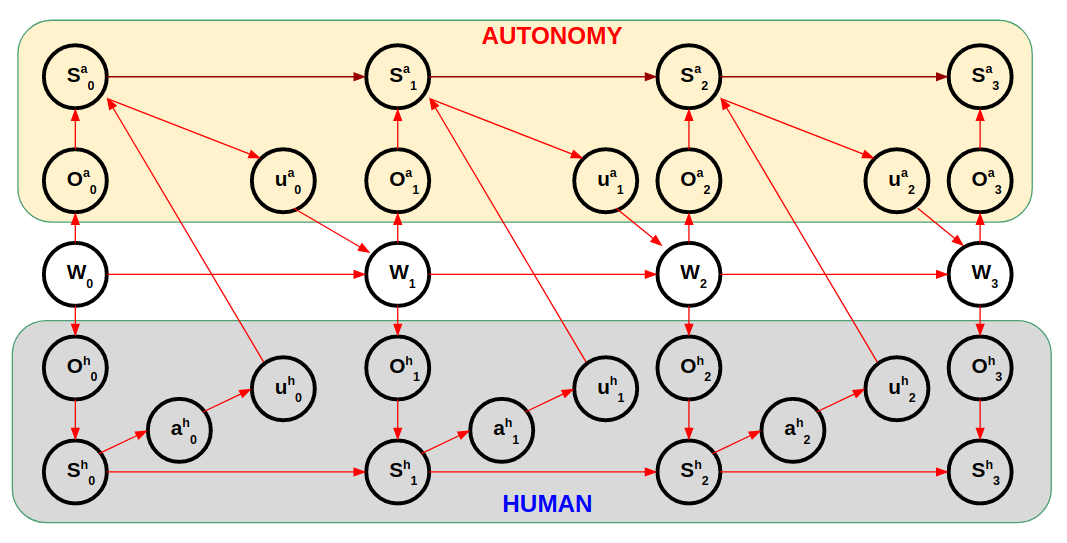
\includegraphics[keepaspectratio, width = 1\textwidth, center]{./figures/pa_loop.png}
	\caption{Our model of Human-Autonomy Interaction as a coupled perception-action loop that unfolds in time represented as a Causal Bayesian Network. The nodes represent various relevant variables that interact with each other at discrete time steps. $\textbf{w}_t$ refers to the robot state. $\textbf{s}^h$ and $\textbf{s}^a$ denote the internal state of the human and autonomy respectively. $\textbf{o}^h$ and $\textbf{o}^a$ refer to the noisy observations of the true robot state that are accessible to the human and autonomy respectively. $\textbf{a}_h$ represents the action taken by the human and $\textbf{u}_h$ denotes the human control command as filtered through a control interface such as a joystick. $\textbf{u}_a$ represents the autonomy's control command. The evolution of robot state is governed by the stochastic dynamics of the environment.}
	\label{fig:cbn}
\end{figure}
Once modeled as a coupled perception-action loop HAI lends itself perfectly to information-theoretic analysis by which we can quantify the \textit{information dynamics} that unfolds during interaction in a mathematically concrete fashion. Once quantified, design of autonomy can be accomplished with an aim of \textit{shaping} the information flow in the joint system towards desired specifications to achieve desired outcomes.  By characterizing the information dynamics in HAI using the proposed framework, we seek to:

\begin{enumerate}
	\item Quantify colloquial notions of transparency, cooperation, coordination etc., that are relevant to HAI using information-theoretic notions of directed information flow and transfer entropy~\cite{schreiber2000measuring} that can be computed directly from the statistics of data without the need for domain- and task-specific metrics and models. 
	
	\item Develop a framework that will provide a systematic and principled approach to design of autonomy, in which autonomy is interpreted as appropriately timed \textit{interventions} with an aim to modulate the bi-directional information flow between the human and autonomy thereby facilitating faster inference and learning and enhanced task performance.
	
	\item Bring different aspects of HAI, such as inference, learning, task performance, transparency and cooperation under a single umbrella in order to shed light on the more fundamental and low-level descriptors and characteristics of human-autonomy teaming. 
\end{enumerate}
Information-theoretic measures such as transfer entropy and predictive information have been widely used to quantify information flow between nodes in a Bayesian network to reveal correlational as well as directed causal influence between components of a complex system~\cite{ay2008information}.
%
%Is higher transparency from A to B related to a) A having a causal influence on B's actions b) improving B's ability to predict A's next actions? I think the latter is more efficient. If B can predict A better, this amounts to have a more accurate model for how A will behave. The entropy of A's next action distribution will be lower given more transparent previous actions by A. 
%
%Can information theoretic ideas be used to characterize states of the joint system in which cognitive load on the user and `energy consumed' for various phenomena such as inference (of human goals, deciding on policy)
%
\subsection{Primer on Information Theory}
In this subsection we describe some of the fundamental information theoretic quantities that are essential for the quantification of information flow between nodes of a causal Bayesian Network. 
\subsubsection{Entropy and Mutual Information}
The most fundamental quantity in information theory is \textit{entropy}. For a discrete random variable $X$ the entropy, $H(X)$ is given by
\begin{equation*}
H(X) = -\sum_{x \in \Omega}^{} p(x)\text{log}_{2}~p(x)
\end{equation*}
where $p(x)$ is the probability mass distribution and the summation extends over all possible states the random variable can assume. Entropy can be interpreted as the average uncertainty in the value of a sample of a variable. 
The above definition of entropy for a single random variable can be extended to two variables in a natural way. For random variables $X$ and $Y$ the \textit{joint} entropy is defined as 
\begin{equation*}
H(X, Y) = -\sum_{x \in \Omega_x}^{}\sum_{y \in \Omega_y}^{}p(x,y)\text{log}_2~p(x,y)
\end{equation*}
where $p(x,y)$ is the joint probability distribution and the summation is over all possible values that $(x,y)$ can acquire. This definition can be extended in a similar fashion to an arbitrary number of variables. 

Closely related is also the idea of \textit{conditional} entropy, which is the entropy of a random variable after we have taken into account some context. The conditional entropy of random variable $X$ given $Y$ is defined as 
\begin{equation*}
H(X|Y) = -\sum_{x \in \Omega_x}^{}\sum_{y \in \Omega_y}^{}p(x, y)\text{log}_2~p(x|y)
\end{equation*}

Yet another important information theoretic quantity of interest is \textit{mutual information}. Mutual information is the amount of information \textit{shared} between two random variables $X$ and $Y$ and can be interpreted as the statistical dependence between them. The mutual information $I(X;Y)$ is defined as 
\begin{align*}
I(X;Y) &= \sum_{x \in \Omega_x}^{}\sum_{y \in \Omega_y}^{}p(x,y)\text{log}_2\frac{p(x,y)}{p(x)p(y)} \\
&=  H(X) - H(X|Y) = H(Y) - H(Y|X)
\end{align*}
and can be interpreted as the KL divergence of the product of the marginal distributions from the joint distribution. Furthermore, mutual information is symmetric in its arguments. 

Not surprisingly, the \textit{conditional mutual information}, an information measure crucial for the computation of transfer entropy, is the shared information between two random variables $X$ and $Y$ in the context of a third random variable $Z$. It is given by
\begin{align*}
I(X;Y | Z) &= \sum_{x \in \Omega_x}^{}\sum_{y \in \Omega_y}^{}\sum_{z \in \Omega_z}^{}p(x,y,z)\text{log}_2\frac{p(x,y,z)p(z)}{p(x,z)p(y,z)} \\
&= \sum_{x \in \Omega_x}^{}\sum_{y \in \Omega_y}^{}\sum_{z \in \Omega_z}^{}p(x,y,z)\text{log}_2\frac{p(x|y,z)}{p(x|z)}\\
&= H(X|Z) - H(X|Y,Z).
\end{align*}
\subsubsection{Transfer Entropy}
All the above mentioned measures deal with static random variables. If we want to investigate dynamics of random time-series processes, transition probabilities need to be considered. Let $X$ be a random time-series processes of random variables $\{\dots, X_{n-1}, X_n, X_{n+1}, \dots\}$ with process realizations denoted by $\{\dots, x_{n-1}, x_n, x_{n+1}, \dots\}$, where $n$ denotes the discrete countable time index. Let $\boldsymbol{X}_n^{(k)} = \{X_{n-k+1},\dots,X_{n-1}, X_n\}$ denote the $k$ consecutive variables of $X$ which has realizations $\boldsymbol{x}_n^{(k)} = \{x_{n-k+1},\dots,x_{n-1}, x_n\}$\footnote{$\boldsymbol{x}_n^{(k)}$ are the Takens' \textit{embedding vectors} whose \textit{embedding} dimension is $k$ and represents the \textit{state} of the $k^{th}$ order Markov process. This is due to the Taken's delay embedding theorem which allows for the reconstruction of the underlying state representation of a dynamical system from the time series data.}. 

Now let us consider another random time-series process of random variables denoted by $Y$. We shall refer to $Y$ as the source process and $X$ as the target process. Transfer entropy captures the notion of information transfer between $Y$ and $X$, as the amount of information that the source process provides about $X_{n+1}$ (the target's next state) after considering the target's past states. Therefore, transfer entropy is a directional measure and is asymmetric with respect to the two random processes $X$ and $Y$. The transfer entropy is defined as 
\begin{equation*}
TE_{Y \rightarrow X}(k,l) = \sum_{}^{}p(x_{n+1}, \boldsymbol{x}_n^{(k)}, \boldsymbol{y}_n^{(l)})\text{log}~\frac{p(x_{n+1} | \boldsymbol{x}_n^{(k)}, \boldsymbol{y}_n^{(l)})}{p(x_{n+1}|\boldsymbol{x}_n^{(k)})}
\end{equation*}
where $k$ and $l$ are the embedding dimensions of the target and the source respectively and the summations is over all possible joint configurations for $x_{n+1}, \boldsymbol{x}_n^{(k)}$ and $\boldsymbol{y}_n^{(l)}$. 
Transfer entropy can be expressed in terms of conditional mutual information between the variables as
\begin{equation*}
TE_{Y \rightarrow X}(k,l) = I(X_{n+1}; \boldsymbol{Y}_n^{(l)}|\boldsymbol{X}_n^{(k)}).
\end{equation*}

This particular mathematical form of transfer entropy is important for computational purposes. As is obvious from the equations above transfer entropy values depend on the embedding dimensions. Embedding dimensions are selected to ensure that active information storage (information contained in the past states of the target) is eliminated properly and is not counted in the transfer entropy computation. 

\subsubsection{Estimation from Data}

Although the mathematical expressions for all the information theoretic measures discussed so far in this paper are relatively straightforward and interpretable there are various issues that arise in practice. First of all, the probability densities contained in each of the measures need to be empirically estimated from a finite number of data samples obtained from the time-series of the random process of interest. Any such estimator is prone to bias and variance due to the limited number of samples available. This problem is exacerbated for continuous valued random variables.

One approach to estimate the relevant probability densities is to use \textit{kernel estimators}~\cite{silverman1986density}. The joint probability densities are estimated using a \textit{kernel function} denoted by $\Theta$ which measures the `closeness' of pairs of samples. For example, we can estimate the joint density of two variables as 
\begin{equation*}
\hat{p}_r(x_n, y_n) = \frac{1}{N}\sum_{n^{\prime} = 1}^{N}\Theta\Bigg(\norm{\begin{bmatrix}
	x_n - x_{n^{\prime}} \\
	y_n - y_{n^{\prime}}
	\end{bmatrix}}-r\Bigg)
\end{equation*}  
where $N$ is the total number of samples, $r$ is the kernel width and $\Theta$ is a step kernel such that $\Theta(x > 0) = 0$ and $\Theta(x \leq 0) = 1$ and $\norm{\cdot}$ is the maximum distance. Kernel estimators are model-free and therefore can be utilized to measure nonlinear relationships. 

An improvement upon the kernel-based estimation approach for mutual information was proposed by Kraskov et. al~\cite{kraskov2004estimating}. Their approach combines various techniques that are designed to reduce the bias and variance errors that can occur due to small sample sizes. This approach relies on a nearest-neighbors approach which is effectively equivalent to dynamically changing the kernel width to the density of the samples. 

In the following chapter, I will describe the proposed studies that will be conducted as a part of this thesis. 

\pagebreak
\section{Proposed Studies}
\subsection{Information Theoretic Quantification of  Transparency}\label{study:rq1}

\subsubsection{Introduction}
Transparency in HAI supports efficient, flexible and coordinated interaction and plays a critical role in facilitating higher overall joint performance [ref]. One of the most common interpretations of transparency concerns the \textit{observability} and \textit{predictability} of an agent's behavior [ref]. During HAI in shared autonomy, as the interaction unfolds, the agents partaking in joint task execution continually take different types of actions that affect the environment. Some actions are more transparent than others---that is, some actions make the agent's underlying decision-making logic, internal states and goals more clear to an observer than others. 

Our hypothesis in this experiment is that, in a task in which the agents have a well defined goal (could be a shared goal as well), improvement of transparency (and consequently the predictability) of a single agent's actions can result in increased predictability of other agents' actions as well. That is, if one agent makes an attempt to be more transparent about its internal state and intentions, the other agents (under rationality assumption) will make use of the information that was made available during transparent behavior and act more predictably. That is, higher transparency implies higher predictability of actions and vice versa.  

Our overarching goal in this experiment is to be able to determine the overall transparency levels of human-autonomy interaction in a given task setting directly from sensor measurements. To that end, we propose the use of information theoretic notions of transfer entropy to characterize transparency. 
%
%Agents take actions in the environment → Some actions are more transparent than others.
%
%Core principle: In a joint task setting, when one agent’s actions are more transparent, the predictability of other agent’s actions can also increase. Can transfer entropy capture this increase in predictability?

\subsubsection{Approach}
In order to investigate the potential usefulness of information theoretic ideas to characterize transparency levels in HAI, in this study we focus on robot-to-human transparency. In information theoretic terms, robot-to-human transparency is defined as 
\begin{equation}\label{eq:transp}
\text{transparency}_{A \rightarrow H}(t) = TE_{A \rightarrow H}^{k,l}(t)
\end{equation}
where $k$ and $l$ are the embedding dimensions of the source and the target respectively. 
It has to be noted that autonomy could use different modalities to improve transparency. However, in this study we focus only on robot motion, that is, the autonomy uses \textit{robot motion} as a way to implicitly communicate its intentions and goals. We carefully manipulate two independent factors that directly affect robot motion (and consequently transparency) and observe how it affects the predictability of human actions. 

Note that, transfer entropy computation is typically carried out between two random processes. In the proposed definition of transparency in Equation~\ref{eq:transp} $R$ and $H$ indicate some random processes associated with the autonomy and human and will be dependent on the task and modality used for expressing intent. For example, if the autonomy only uses \textit{robot motion} as a way to communicate its intent we can use the time series associated with robot trajectory, end-effector velocity, directedness towards the end-goal etc., as the source process and time series associated with the user control commands as the target process. 
%
%Robot-To-human transparency. 
%
%Goal: To be able to decipher transparency levels directly from sensor measurements (robot and human control actions)
%
%Idea: Use information theoretic notion of transfer entropy to characterize transparency
%
%Higher transparency = higher predictability of actions. 

\subsubsection{Experimental Design}

The experiment consists of a human subject interacting with a robotic arm that is endowed with autonomous capabilities in the context of a table-top manipulation setting. As our experiment focuses on robot-to-human transparency, in each trial the autonomy has an internal goal (a reaching target) that is unknown to the human. In each trial, the human has to infer the autonomy's goal and teleoperate the robot towards the goal as quickly as possible. 

Transparency of autonomy's actions directly depends on the legibility of robot motion and therefore maximum transparency is achieved when the autonomy drives the robot along a legible path towards the goal without any interruptions. 

In order to modulate the transparency of autonomy's actions we systematically manipulate two independent factors:
\begin{enumerate}
	\item \textbf{Signal dropout}: This factor controls the percentage of the total trial time that the robot is stalled due to nil control commands issued to the robot and as a result creates discontinuity in the robot's motion. 
	\item \textbf{Direction of end-effector motion}: Any deviation from the legible path can potentially affect the transparency of autonomy's actions. The higher the deviation as a result of a perturbation to the the control commands issued to the robot higher will be the impact on transparency. In this system, the perturbation is generated using a zero-mean Gaussian noise added to the end-effector velocity. 
\end{enumerate}

At the end of each trial, subjective evaluation of transparency of autonomy's actions will also be collected via questionnaires so that correlation analysis can be performed between the transfer entropy-based transparency measure and the subject's perception of transparency. 

The autonomy's policy is 	

Before the testing phase, subjects will undergo a short training phase during which they will observe unimpeded legible robot motion towards various targets on the table. This is done to ensure that the human has a sufficiently good model of how the autonomy will accomplish the reaching task.  
The core hypothesis we seek to test in this study is that \textit{in trials with higher transparency, the user actions (control commands issued via the interface) will be more predictable and therefore transfer entropy from robot state to user command will be higher. }

%
%Experiment Protocol:
%\begin{enumerate}
%	\item Autonomy has an intended goal (unknown to human). Autonomy tries to move the robot towards the goal using a straight line path policy(?) (Sid’s suggestion. Prior work has shown ‘legible motion’ is what conveys transparency via motion. So use legible motion instead of straight line. For some goal configuration legible will be same as straight line. Implementation issues - I want legible velocity space policies. Not path planned trajectories. )
%	
%	\item Human has to infer autonomy’s goal and teleoperate the robot towards the goal. How to establish ground truth. Michael’s idea was to have a pilot study where people are just evaluating how transparent the robot actions ‘look like’. The next stage would be to study how humans act in the presence of autonomy having different levels of transparent behavior.
%	
%	\item Systematic manipulation of two factors that can direct affect the transparency of autonomy's intent when controlling the robot, namely, signal sparsity and directional perturbation. Subjective evaluation of transparency for each trial for correlation analysis. 
%	
%\end{enumerate}
%
%Hypothesis → In trials with higher transparency, the user command will be more predictable and therefore TE from robot state to user command will be higher.

%
%
%Caveats: It is possible that EVEN when one agent tries to be more transparent the other agent does not pick up on those cues and therefore will likely continue to act in an unsure manner? Therefore transparency is not just a property of how one agent acts. But it is also about how the other agent receives and interprets those actions and uses them to inform their own actions

 
%
%
%
%Training phase
%
%Online computation of policy. Iterative Optimal Control. Probably needs GPU to perform fast Optimal control. 
%
%Evaluation: Measure task related metrics, Measure subjective metrics. Ask= about perceived transaprency level. Evaluate whether having the robot strive for maximizing transparency results in better task related metrics. 

\subsection{Guided Active Learning in Humans}\label{study:rq2}
\subsubsection{Introduction}

In the context of shared autonomy for assistive robots, the users typically still have some amount of control over the robot at all times. The primary job of autonomy assistance is to supplement or in some cases complement the users' capabilities in order to improve overall objective and subjective task performance. If it is the case that the users are not adept at controlling the robot on their (within the constraints they have due to motor impairments or control interface), then the effectiveness of having assistance is typically not very high. That is, it beneficial for the overall system that the users have a high level of skill in teleoperating a robot. 

However, high-dimensional robot control using low-dimensional control interfaces is not an easy task. Users gain experience and progressively become better at robot control via trial and error.

In this study, I am interested in exploring how autonomy can help the human in this learning process. I am inspired by ideas of curriculum learning in which a learner (could be an animal or an artificial machine learning system) learns about a training distribution or a hypothesis by exploring a set of examples following a systematic curriculum, typically by experiencing `easy' examples first followed by the harder ones. 
%
%
%Assistive robotics, people control robots using control interface. Autonomy is added to these robots to make life easier. In many cases this would still require the user to teleoperate the robot.
%
%Controlling a robot is typically not an easy task for a user. The user is presented with a few different learning problems when they are faced with the task of learning how to control the robot

%In this study, I am interested in exploring how autonomy can help the human user learn the dynamics of the robot more effectively. I am inspired by ideas from curriculum learning in which learner (could be a human or a machine learning system) learns about the training distribution (is this same as learning system dynamics of an unknown physical system) by exploring the training set following a systematic curriculum, typically by learning `easy' examples first followed by harder ones. 

Our previous studies have shown us that when humans learn to control a robotic arm using a standard control interface, they are faced with different types of learning problems, some of which are,
\begin{enumerate}
	\item They need to learn how to activate the control interface. For example, how to `press' a button, how to `push' a joystick etc,.
	\item They need to learn what the control mappings are 1) That is, upon pushing the joystick forward, which direction is the robot going to move. This also requires implicit learning of the reference coordinate systems as well as the associated coordinate transformations. 
	\item They need to learn a forward model that predicts the next state of the robot given the current state and action taken. This is more specific than the previous point. Learning the forward model will require understanding of reference coordinate frames and transformations as well. 
	\item They need to learn an inverse model that can generate an action given the current state and a desired next state. This is essential if the robot is to be used for performing specific tasks. 
\end{enumerate}
Self-guided learning process can potentially have the following issues:
\begin{enumerate}
	\item During the training phase users might not necessarily explore different parts of the state space properly. As a result of which the nonlinearities in the kinematics are not properly understood. Nonlinearities are dominant typically near the edges of the workspace or near self-collision configurations. 
	\item It is also likely that during the self-guided training phase users' don't experience what we call `cognitively hard states'. Cognitively hard states are defined as those in which the inverse control problem takes more cognitive and computational resources. The difficulty likely arises due to the complexity of coordinate transformations involved. 
\end{enumerate}

In this study, I am primarily interested in the design of a curriculum that will make the training phase more effective. We propose an algorithm for automatically generating a curriculum for the user's training phase. The autonomy, in this framework, plays the role of an informative teacher that presents the user with scenarios such that subsequent practice in and around the scenario results in maximal skill acquisition. 
%
%Core Questions"
%\begin{enumerate}
%	\item How can we design a curriculum so that the training phase is most effective? Need to define what effective is. Effectiveness as measured by the improvement in skill level at the end of the training phase. How to measure skill level (or improvement in skill level? ). Have the subjects perform a wide variety of tasks that require them to use different types of kinematics skills with the robot. 
%	\item The automatic procedure of generating curriculum is framed as assistance provided by the autonomy. The autonomy plays the role of an informative teacher who provides examples(?) or presents the learner with scenarios such that the skill acquisition is maximized. Should the skill acquisition be a general thing or should it be task-specific skill acquisition. 
%	\item The exact procedure of how a human learns how to control a robot might involve some exploration some trial and error and learning from errors. Let us explain out how people typically explore the control space and the state space. (Is this a general phenomena, we need to clarify this via experiments and doing data statistics)
%	THIS IS IMPORTANT BECAUSE, BEFORE WE COME UP WITH IDEAS FOR HOW TO HELP PEOPLE LEARN, WE NEED TO UNDERSTAND HOW PEOPLE LEARN. (Could BMI learning be a good testbed for this?)
%	
%	
%	The robot is at some arbitrary starting position. The user is instructed that the control commands perform tranlsation with respect to the world frame and the orientation is with respect to the hand frame. It is possible that the user does not fully understand what this means until s/he explore the control and command space properly. 
%	
%	Exploring the control space - can possibly be considered as learning the inverse controller (Or is it?) 
%	
%	Exploring the state space - can possibly be considered as learning how being in different parts of the state space changes how the robot responds to the same control command. Thereby getting insight into the nonlinearities in the robot kinematics. 
%	
%
%\end{enumerate}
%
%Typical exploration might proceed as follows: The user will cautiously move the joystick is some direction and observe how the robot moved. User might most likely pick axis directions as defined by the interface (which the user was told beforehand) and to see what it does to the robot (that is, how the robot moves). Might start with smaller movements progressively increasing to bigger movement (not necessarily, depends on how cautious the user is?). We are assuming that this exploration is task-free. One of the questions is whether the user typically comes back to the `starting position' after exploring each dimension so that the baseline is always the same. This is possibly where the user might miss out on experiencing cognitively harder states. By coming back to the starting position every time, the users are effectively freezing $x_t$ in the tuple ($x_{t+1}, x_t, a_t$) thereby they can delineate how different actions can affect the present (a single) state. 
%
%There are cognitively hard states: most likely this arises due to the complexity of coordinate transformation that is involved. And then there are nonlinearities in kinematics: which arise typically due to the physical constraints of the robot (such as at the edges of the workspace or near self-collision zones). Workspace limits are the primarily reason why there are kinematic singularities. As the manipulability of the robot arm is lower near workspace singularities, typically these configurations are not highly useful for properly accomplishing tasks. That is, the `empowerment' offered by these configurations are typically low. 
%
%
%
%In this study, we will design an algorithm in which the autonomy will guide the human in the process of learning 
\subsubsection{Approach}
The first step towards the design of a teaching curriculum is to quantify how self-guided learning proceeds and identify room for improvement. To this end, our first goal is to understand the temporal and spatial statistics of how humans explore the robot's workspace during training. We will use a collection of observations from multiple instances of state space during self-guided training to generate an \textit{information density map} $\phi_{1}(\boldsymbol{x})$. This information map will shed light on the relative importance that users give to different parts of the workspace during the exploration process. Similarly, an information density map could be generated from data collected during task execution (denoted as $\phi_{2}(\boldsymbol{x})$) which will reveal `cognitively harder states' as it is possible that users will spend more time in cognitively hard regions. 

In this framework, we view the process of learning to control a robot as a special case of motor learning in which there is a flow of information from the unknown function (nonlinear kinematic function that governs the time evolution of the robot's kinematic state) to the user's internal representation of the function. The goal of the algorithm is to present the user with examples such the user gain maximal information regarding the underlying unknown function (or in other words, will maximally reduce the entropy). The goal of the algorithm is to drive the user's exploration trajectory towards those parts of the state-space that are typically not explored during self-guided training to regions which users typically find to be cognitively harder. That is, we want the user's trajectory to be ergodic with respect to the combined information density map, $\phi_{2}(\boldsymbol{x}) - \phi_{1}(\boldsymbol{x})$

We will use the combined information density map to characterize the different regions of the workspace and different `training zones' will be sampled according to the information density map during the training phase. The autonomy will then nudge the user to explore the robot kinematics in and around the chosen training zones such that the exploration trajectory becomes maximally ergodic with respect to the combined information density map. By having the user spend more exploring regions of the state space that are typically not explore and are cognitively hard, the hypothesis is that they will have a better understanding of robot kinematics and control throughout the workspace and thereby will be able to perform a wider variety of tasks more skillfully. 
% 
%Fundamental problem:
%
%There are cognitively hard states. These configurations are one in which, given the target configuration, the user takes more time in responding with the correct action signal. Or there is a high likelihood that the user makes errors initially and relies on online feedback to generate the correct control signal. Eventually, the user might be able to get better with practice. This is under that assumption that the user knows how to do 1) and that the main issue is in 2). 
%
%We want autonomy to be able to identify these cognitive hard states and then during the training phase would want to guide the user to explore the state space region around these cognitively hard spots so that when test time comes, users don't struggle. This is so that users get to practice and experience those states and state transitions that are cognitively harder so that the teleoperation performance is normalized across different parts of the state space. 
%How can autonomy help. 
%
%Autonomy can nudge the user to explore regions of state space that are cognitively hard/rarely accessed that possess high degree of nonlinearities. The autonomy can guide the robot to such regions and then prompt the user to explore robot control in those regions. 
%
%Learning to control a robot using a joystick can be thought of function learning/motor learning? Can learning be thought of as information flow from an unknown function to the user's internal representation of the the function. (Reference this)
%
%More time a user spends exploring a part of the state space, it is likely that they would become more comfortable in controlling the robot in that region. How the user explores the state space can be quantified using a measure of ergodicity? Ergodic measure can characterize the exploration pattern and can possibly expose which regions are not explored by humans typically. 
%
%Get a bunch of people. Have them teleoperate the robot from a specific start state to end state? Charcaterize which ones are harder. This would give us an idea of what are cognitively hard states. Possibly can extrapolate between known points using some sort of metamodeling techniques? 

\subsubsection{Experiment Design}
The information density map described in the previous section will be generated by combining exploration during training data from multiple subjects offline. For the study, the subjects will be divided into two groups, A and B. 

Subjects in Group A will undergo a training phase in which the training zones will be sampled from a uniform information density map. Whereas, the training zones for Group B's will be sampled according to the information density map generated from ergodic measures of self-guided exploration process. 

After the training phase, the subjects will undergo a testing phase in which their skills will be put to tests. The subjects will perform a wide variety of reaching tasks that will require complex control of the robotic arm. 

The core hypothesis is that \textit{subjects in Group B will have outperform subjects from Group A in the testing phase as a result of better understanding of robot control in cognitively hard states due to a systematic training curriculum chosen by the autonomy.}

\subsection{Optimizing Task Performance}\label{study:rq3}

\subsubsection{Introduction}
Design of autonomy for a shared-control system ideally should focus on HAI that improves task performance and safety, increases user satisfaction and acceptance. One of the most critical factors that contributes to overall performance of a human-robot team is transparency of interaction. That is, knowledge of \textit{why}, \textit{how} and \textit{what} each other agent is doing can lead to better interaction. 

In this study, we seek to concurrently improve
different aspects of HAI (both subjective and objective task metrics) by optimization of a more low-level aspect of interaction such as that of  \textit{transparency}. The hypothesis is that optimization of bi-directional transparency will likely result in better communication of latent internal states. By leveraging the fact that human actions can be influenced by robot actions, robot policy can be designed in such a way that it drives the joint human-autonomy system to states with higher transparency. This will result in a common ground~\cite{kiesler2005fostering} for joint task execution, which will lead to enhanced cooperation, coordination and mutual trust. As a result of these enhancements, the desired objective and subjective outcomes will naturally emerge.

%By leveraging the fact that human actions can be influenced by robot actions, robot policy can be designed in such a way that it drives the oint human-autonomy system to states with higher transparency. As a consequence, task related metrics such as task completion time, number of mode switches, and subjective task metrics such as perceived trust, satisfactoin etc can simulatenously be enhanced. 

\subsubsection{Approach}
In this study the generation of autonomy policy is framed as optimal control problem. More formally, the objective is to determine an autonomy control signal 
$u_r^t \;\;\forall \;\; t \in [0, T]$ such that $\int\limits_{0}^{T} TE_{R \rightarrow H}^{k, l}(t)$ is maximized. That is, the optimal solution for the robot control signal will maximize transparency from autonomy to human. This optimization will be done using an iterative Model Predictive Control framework. In order to do MPC successfully, we will require different types of models. 

First of all, we will require a robot dynamics/kinematics model given by $x_r^{t+1} = f_{\boldsymbol{\Theta}}(x_r^t, u_f^t)$. For simple robots, the kinematics could possibly be expressed as analytical functions. For more complex robots, the kinematic models could be learned directly from data using different techniques such as deep neural networks or Koopman Operators. 

Second of all, we will require a model for the policy implemented by the human. It has been established in prior work that humans act differently in the presence of autonomy. Therefore, in this work we are specifically interested in a model that will help us predict user actions in the presence of autonomy. This model can be thought of an inverse controller that the user implements to generate actions in a given context and can be written as $u_h^{t} = p_{\boldsymbol{\eta}}(x_r^t, u_r^t, g^t)$ (and possibly history of these variables as well) where $\boldsymbol{\eta}$ represents the model parameters. Similar to the robot kinematics model, the human action prediction model can also be learned from data.

Lastly, we would also need an arbitration function that will determine how the user control command and autonomy control command will be arbitrated. The arbitration function $\beta$ will generate $u_f^t$ given by $u_f^t = \beta_{\boldsymbol{\alpha}}(u_r^t, u_h^t)$, where $\boldsymbol{\alpha}$ represents the model parameters. 
%
%%
%%Goal: To generate robot policy that will drive the joint HA system towards higher transparency state.
%
%What's needed: Robot dynamics model. $x_r^{t+1} = f_{\boldsymbol{\Theta}}(x_r^t, u_f^t)$, Human action model in the presence of autonomy $u_h^{t+1} = p_{\boldsymbol{\eta}}(x_r^t, u_r^t, g^t)$ (and possibly history of these variables as well) this can be learned from data. Arbitration function $u_f^t = \beta_{\boldsymbol{\alpha}}(u_r^t, u_h^t)$ (could possibly be a fixed function).
%
%Optimal control framing. objective is to determine $u_r^t \;\;\forall \;\; t \in [0, T]$ such that $\sum_{t=0}^{T} TE_{R \rightarrow H}^{k, l}(t)$ is maximized. 

\subsubsection{Experiment Design}

The robot kinematics model and the human action prediction model will be trained offline prior to individual subject sessions. The model performance will be evaluated using standard cross validation techniques that are widely employed in the domain of machine learning. 

Each session will consist of a training phase and a testing phase. During the training phase, the subject will get accustomed to the control interface and the control mappings and gain experience controlling the robotic arm. 
During each session, subjects will control the assistive robotic arm to perform simple reaching tasks in a shared control setting. Two conditions will be tested: (condition A) one in which the autonomy signal is generated using a simple distance based optimizer (straight line potential field) and the other (condition B) will use the optimization procedure described in the previous subsection. 

We seek to investigate how task related objective metrics as well as subjective metrics differ between the condition A and B. The core hypothesis is that \textit{for trials utilizing condition B the perceived transparency levels will be higher and as a result both subjective and objective metrics such as will likely be better. } In order to collect data regarding perceived transparency levels, we will have the subjects fill out a survey after every trial. 

%The
%Group A: Does free exploration? or randomly chosen points in the state space for exploration
%
%Group B: Points in state space are chosen according to ergodic measures that characterizes typical human exploration patterns (and thereby the holes in the exploration) or points in state space that correspond to cognitively harder states. 
%
%For each group have the user explore these points for more time. 
%
%Then have them do tasks. 
%
%Group A, might struggle, because teleoperation might be hard and as a result task performance might be bad. 
%
%Group B, since the practice routine was good, the user might be better prepared for dealing with the complex control that are required of certain types of tasks. 

%\subsection{Task Performance}

%\subsection{Aspects of HRI}
%
%Softer aspects of HRI that are studied. Prescriptive models for HRI. 
%
%What makes HRI more 'natural' and fluid?
%
%The need for communication is established in 22 and 24 reference.  in Nikolaidis and Julie Shah
%Importance of legibility, communication, information exchange, transparency etc. 
%
%GUY HOFFMAN - FLuency. Fluency metrics. Do they all have an information theoretic angle to them?
%
%Joint attention. Initiating, responding, and ensuring. Relate joint attention processes to information transfer. Joint attention is related to transparency. If there is some sort of connection between joint attention and information flow then transparency is also related to informatoin flow between agents. 
%
%Transparency related papers. Opinion articles.
%
%Charcaterization of HRI paper. REview papers.  
%
%Lyons and Havig Paper. Models for transparency.
%
%USer- centric system development to prioritize user preferences etc. My paper RSS 2016, Wheelchair paper HRI Social psychology. Proxemics.
% 
%\subsection{Causal Bayesian Networks for Modeling HRI}
%
%
%Notion of perception action loops as expounded in the review paper. Shared control vs. Traded control. 
%Living beings, robotic systems as agents perceiving and acting upon the environment. 
%
%Perception Action Loop. Constant exchange of information between agent and environment. Reference to Klyubin's work. 
%Specify how is it different from my proposal. 
%Page 8 in Capdeduy Thesis. 
%
%How information is accessed, stored and processed becomes important for the emergence of cognitively sensible behavior. \textit{Empowerment} has been looked at. 
%
%Multiple agents imply that there are multiple perception action loops interacting and co-existing. Environment of one agent will includes the other agents. 
%
%Multi-agent systems as a multi coupled perception action loops. Reference Philip Capdeduy's work. 
%
%Philip Capdeduy looks into this idea in the context of multiple artificial agents. Here we are adopting it to the case of human-robot interaction. 
%
%Bayesian Networks and Causal Bayesian Networks. 
%
%Coupled PA loops are Causal Bayesian Networks. Reference Klyubin, Polani et al. 
%
%Identify the nodes. Give an example model (This would look like the content in Klyubin et al. ). Identify different subnetworks as intuitive components of an HRI system. Ground the learning, inference and task performance problem by relating it to either inferring on improving some aspect of the network. 
%
%Introduce notions of information flow and why it would be useful in this context? What does it correspond to. 
%
%Introduce the notion of intervention in the sense of Judea Pearl and make a distinct. 
%
%Connect autonomy design to intervention and autonomy as a way to manipulate information flow 
%
%\subsection{Information Theory and Flow in CBNs}
%
%Short chapter that serves as the primer for information theory. 
%
%Basic concepts of entropy, joint entropy, cross entropy, mutual information, transfer entropy, information flow in CBNs. 
%
%After mathematical introduction of the above-mentioned concepts justify why these metrics are 
%
%Information as a currency of life? Polani ideas?
%
%
%\pagebreak
%\section{Proposed Work}
%\subsection{Inference}
%Different types of inference. Make inference easier by becoming more legible, transparent. Bidirectional intent inference. We are focused on human to machine. DEvelop information theoretical framework for goal disambiguation. 
%\subsubsection{Related Work}
%\subsubsection{Experiment Design}
%\subsection{Learning}
%Guided Active Learning. Where the autonomy is the guide. Human do active learning (tinkering) on their own. Autonomy, plays the role of a teacher/guide and guides the active exploration so that the rate of learning is higher for the human. 
%\subsubsection{Related Work}
%\subsubsection{Experiment Design}
%\subsection{Task Performance}
%\subsubsection{Related Work}
%\subsubsection{Experiment Design}
%
%\section{Timeline}
%\begin{table}[hc]
%\begin{small}
%\begin{center}
%\begin{tabular}{lll}
%Timeline & Work & Progress\\
%\hline
%          & XXXXXXXXXXXXXXXXXXXXXXXXXXXXXXXXXXXXX & completed\\
%Nov. xxxx & XXXXXXXXXXXXXXXXXXXXXXXXXXX & ongoing\\
%Jan. xxxx & Thesis writting & \\
%Feb. xxxx & Thesis defense & \\
%\end{tabular}
%\end{center}
%\end{small}
%\caption{Plan for completion of my research}
%\label{tab:plan}
%\end{table}
%
%Thus, I plan to defend my thesis in XXX XXXX.

\pagebreak
\section{Timeline}
\subsection{Plan for Completion of Research}
\begin{center}
	\begin{tabular}{ m{5cm}  m{8cm} m{3cm} } 
		Timeline & Work & Progress \\
		\hline
		
		May 2019 & RAL-IROS Submission & Ongoing \\
		
		May 2019 & Thesis Proposal & Ongoing \\ 
		May 2019-September 2019 & Survey Paper & Planning \\
		September 2019 - Jan 2020 & Section~\ref{study:rq1} Paper Submission & Planning \\ 
		
		 Jan 2020 - March 2020 & Section~\ref{study:rq2} Conference Submission  & Planning \\
		 
		 March 2020 - December 2020 & Section~\ref{study:rq3} Conference + Journal Submission  & Planning \\
		 
		 January 2021 & Begin Thesis writing & \\
		 April 2021 & Submit Draft of thesis & \\
		 May 2021 & Revise and Defend! & \\
		  
		\hline
	\end{tabular}
\end{center}
\begin{footnotesize}
\bibliographystyle{plain}
\bibliography{references}
\end{footnotesize}

\end{document}


